%%%%%%%%%%%%%%%%%%%%%%%%%%%%%%%%%%%%%%%%%%%%%%%%%%%%%%%%%%%%%%%%%%%%%%%%%%%%%%%%%%
\begin{frame}[fragile]\frametitle{}

\begin{center}
{\Large Information Extraction}
\end{center}
\end{frame}

%%%%%%%%%%%%%%%%%%%%%%%%%%%%%%%%%%%%%%%%%%%%%%%%%%%%%%%%%%%
\begin{frame}[fragile]\frametitle{}

\begin{center}
{\it ``The task of Information Extraction (IE) involves extracting meaningful information from unstructured text data and presenting it in a structured format.''}
\end{center}
\end{frame}


%%%%%%%%%%%%%%%%%%%%%%%%%%%%%%%%%%%%%%%%%%%%%%%%%%%%%%%%%%%
\begin{frame}[fragile]\frametitle{Example}

We can extract the following information from the text:


\begin{center}
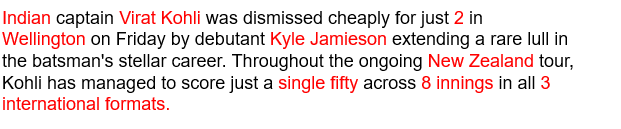
\includegraphics[width=0.8\linewidth,keepaspectratio]{ie13}
\end{center}


	\begin{itemize}
	\item Country – India, Captain – Virat Kohli
	\item Batsman – Virat Kohli, Runs – 2
	\item Bowler – Kyle Jamieson
	\item Match venue – Wellington
	\item Match series – New Zealand
	\item Series highlight – single fifty, 8 innings, 3 formats
	\end{itemize}

Makes text structured meaning with relationships (key value).

{\tiny (Ref: Hands-on NLP Project: A Comprehensive Guide to Information Extraction using Python - Aniruddha Bhandari)}

\end{frame}


%%%%%%%%%%%%%%%%%%%%%%%%%%%%%%%%%%%%%%%%%%%%%%%%%%%%%%%%%%%
\begin{frame}[fragile]\frametitle{}

\begin{center}
{\Large Information Extraction Use case}
\end{center}
\end{frame}

%%%%%%%%%%%%%%%%%%%%%%%%%%%%%%%%%%%%%%%%%%%%%%%%%%%%%%%%%%
\begin{frame}[fragile]
  \frametitle{As a Task}
\begin{center}
\includegraphics[width=\linewidth,keepaspectratio]{ie1}
\end{center}
\end{frame}


%%%%%%%%%%%%%%%%%%%%%%%%%%%%%%%%%%%%%%%%%%%%%%%%%%%%%%%%%%
\begin{frame}[fragile]
  \frametitle{Task}
\begin{center}
\includegraphics[width=\linewidth,keepaspectratio]{ie2}
\end{center}
\end{frame}


%%%%%%%%%%%%%%%%%%%%%%%%%%%%%%%%%%%%%%%%%%%%%%%%%%%%%%%%%%
\begin{frame}[fragile]
  \frametitle{Extraction}
\begin{center}
\includegraphics[width=\linewidth,keepaspectratio]{ie3}
\end{center}
\end{frame}

%%%%%%%%%%%%%%%%%%%%%%%%%%%%%%%%%%%%%%%%%%%%%%%%%%%%%%%%%%
\begin{frame}[fragile]
  \frametitle{Techniques}
\begin{center}
\includegraphics[width=0.8\linewidth,keepaspectratio]{ie4}
\end{center}
\end{frame}

%%%%%%%%%%%%%%%%%%%%%%%%%%%%%%%%%%%%%%%%%%%%%%%%%%%%%%%%%%
\begin{frame}[fragile]
  \frametitle{Example}
\begin{center}
\includegraphics[width=\linewidth,keepaspectratio]{ie5}
\end{center}
\end{frame}

%%%%%%%%%%%%%%%%%%%%%%%%%%%%%%%%%%%%%%%%%%%%%%%%%%%%%%%%%%
\begin{frame}[fragile]
  \frametitle{Landscape of Information Extraction}
\begin{center}
\includegraphics[width=\linewidth,keepaspectratio]{ie6}
\end{center}
\end{frame}

%%%%%%%%%%%%%%%%%%%%%%%%%%%%%%%%%%%%%%%%%%%%%%%%%%%%%%%%%%
\begin{frame}[fragile]
  \frametitle{Complexity of Information Extraction}
\begin{center}
\includegraphics[width=\linewidth,keepaspectratio]{ie7}
\end{center}
\end{frame}

%%%%%%%%%%%%%%%%%%%%%%%%%%%%%%%%%%%%%%%%%%%%%%%%%%%%%%%%%%
\begin{frame}[fragile]
  \frametitle{Applications of Information Extraction}
  \begin{itemize}
    \item Extract structured data out of electronically-available scientific literature, especially in the domain of biology and medicine 
    \item Legal documents
    \item Business intelligence
    \item Resume harvesting
    \item Media analysis
    \item Sentiment detection
    \item Patent search
    \item Email scanning
  \end{itemize}
\end{frame}

%%%%%%%%%%%%%%%%%%%%%%%%%%%%%%%%%%%%%%%%%%%%%%%%%%%%%%%%%%
\begin{frame}[fragile]
  \frametitle{Architecture of Information Extraction}
\begin{center}
\includegraphics[width=\linewidth,keepaspectratio]{ie8}
\end{center}
\end{frame}

%%%%%%%%%%%%%%%%%%%%%%%%%%%%%%%%%%%%%%%%%%%%%%%%%%%%%%%%%%
\begin{frame}[fragile]
  \frametitle{Main tasks of Information Extraction}
  \begin{itemize}
    \item Named Entity Recognition (Chunking, Parsing)
    \item Relation Extraction 
    \item Relations like subject are syntactic, relations like person, location, agent or message are semantic
  \end{itemize}
	

\begin{center}
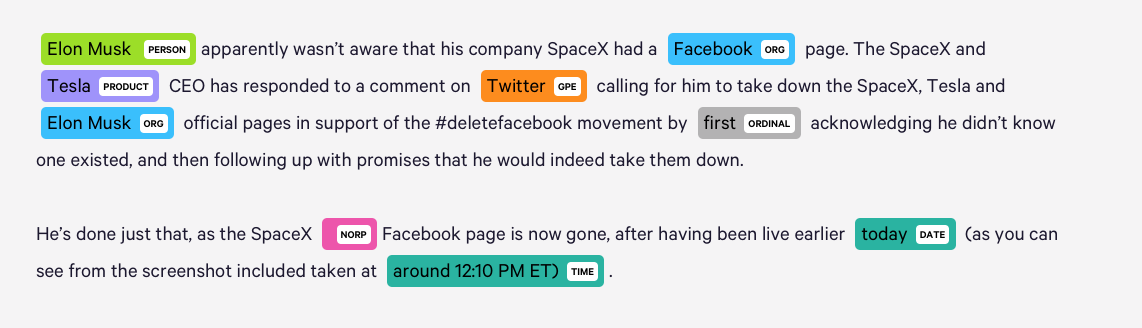
\includegraphics[width=0.8\linewidth,keepaspectratio]{ie14}
\end{center}

\end{frame}

%%%%%%%%%%%%%%%%%%%%%%%%%%%%%%%%%%%%%%%%%%%%%%%%%%%%%%%%%%
\begin{frame}[fragile]
  \frametitle{Example of Information Extraction}
Text:
  \begin{itemize}
    \item Stress is associated with migraines 
    \item Stress can lead to loss of magnesium 
    \item Calcium channel blockers prevent some migraines 
    \item Magnesium is a natural calcium channel blocker
  \end{itemize}
\end{frame}

%%%%%%%%%%%%%%%%%%%%%%%%%%%%%%%%%%%%%%%%%%%%%%%%%%%%%%%%%%
\begin{frame}[fragile]
  \frametitle{Extract semantic entities from text}
\begin{center}
\includegraphics[width=\linewidth,keepaspectratio]{ie8}
\end{center}
\end{frame}

%%%%%%%%%%%%%%%%%%%%%%%%%%%%%%%%%%%%%%%%%%%%%%%%%%%%%%%%%%
\begin{frame}[fragile]
  \frametitle{Classify relations between entities}
\begin{center}
\includegraphics[width=\linewidth,keepaspectratio]{ie10}
\end{center}
\end{frame}

%%%%%%%%%%%%%%%%%%%%%%%%%%%%%%%%%%%%%%%%%%%%%%%%%%%%%%%%%%
\begin{frame}[fragile]
  \frametitle{Do reasoning: find new correlations}
\begin{center}
\includegraphics[width=\linewidth,keepaspectratio]{ie11}
\end{center}
\end{frame}

%%%%%%%%%%%%%%%%%%%%%%%%%%%%%%%%%%%%%%%%%%%%%%%%%%%%%%%%%%
\begin{frame}[fragile]
  \frametitle{Do reasoning: infer causality}
\begin{center}
\includegraphics[width=\linewidth,keepaspectratio]{ie12}
\end{center}
\end{frame}



